%*****************************************
\chapter{The Hybrid Localisation Algorithms} %Hybrid Monte Carlo and Bounded-error Localisation}
\label{ch:implementation}
%*****************************************

In this chapter we will describe in detail the four new hybrid localisation algorithms, the key idea of which is to only perform Monte Carlo localisation over a delimited region of the search space that is constituted of feasible robot positions. This delimited region is determined using the two bounded-error estimators \texttt{HC4} and \texttt{SIVIA}, as described in Section \ref{sec:contractors} and \ref{sec:sivia}, respectively. Thus, by increasing the particle density in interesting regions, the localisation accuracy should increase. Specifically, we will present

\begin{itemize}
	\item a bootstrap particle filter with \texttt{HC4} contractor (\texttt{PFC}),
	\item an unscented particle filter with \texttt{HC4} contractor (\texttt{UPC}),
	\item a bootstrap particle filter with \texttt{SIVIA} (\texttt{PFS}),
	\item and an unscented particle filter with \texttt{SIVIA} (\texttt{UPFS}).
\end{itemize}

\noindent
Depending on the amount of available information in terms of the number of visible landmarks, the delimited region may still be large. Therefore, in addition to the simple bootstrap particle filter, which is simply denoted as particle filter in the following, an unscented particle filter was employed in combination with the respective bounded-error estimator.

As described in Section \ref{sec:unscented_particle}, the unscented particle filter can move particles to regions of the search space that are associated with a high observation likelihood and therefore potentially improve the estimation accuracy, especially when dealing with very accurate measurements. As no particles remain in regions where they would receive an insignificantly low importance weight and therefore simply die in the next resampling step, it may also be possible to further reduce the number of particles, when compared to the particle filter. Finally, the speed of convergence should be influenced positively by actively moving particles towards the peak of the likelihood function.

In a symmetric environment both conventional probabilistic filters may possibly converge to the wrong place and may not be able to recover from this. Using geometrical considerations of the environment, which are further explained below, as well as basic plausibility considerations, convergence to the wrong position can be prevented by excluding the opposing solution from the set of feasible solutions and therefore bringing the initial particles closer to the peak of the true posterior distribution.

A fundamental concept that we will need for the introduction of the state-space and bounded-error model in Section \ref{sec:prob_model} and \ref{sec: bounded_error}, respectively, is the attitude of a robot, which we will elaborate on in the following section. In Section \ref{sec: constraint-filters}, we show how constraints are incorporated in the inherently unconstraint generic particle filter framework. Finally, the four new localisation algorithms are presented in Section \ref{sec:new_filters}.




\section{Attitude Representation}

The orientation of the coordinate frame of a robot, referred to as the \emph{body frame}, with respect to a reference coordinate frame, termed the \emph{world frame}, is known as \emph{attitude}. The origin of the body coordinate system is usually chosen to be the robot's center of gravity. Establishing correspondence between the two frames is one of the goals of the localisation process. In the following section, we will introduce a common attitude representation known as Euler angles.

\subsection{Euler Angles}

Euler angles are one of several mathematical ways to describe the attitude of an object in three-dimensional Euclidean space. They represent a sequence of three elemental rotations about the axes of the world coordinate system, defined as follows:

\begin{itemize}
\item The \emph{roll angle} $\phi$ determines the rotation around the $x$-axis.
\item The \emph{pitch angle} $\theta$ determines the rotation around the $y$-axis.
\item The \emph{yaw angle} $\psi$ determines the rotation around the $z$-axis.
\end{itemize}

\noindent
Figure \ref{fig:Euler_angles} depicts the rotation about the axes $z, y', X$ by $\psi, \theta, \phi$, respectively, according to the Tait-Bryan convention. The colour blue indicates the world frame $\{x, y, z\}$, which matched the body frame $\{X, Y, Z\}$ before the rotations. The colour red indicates the orientation of the body frame after the rotations were carried out. In contrast to \emph{extrinsic rotations}, where each of the three elemental rotations may occur about the axes of the original coordinate system, the Tait-Bryan rotations are \emph{intrinsic rotations} that occur about the axes of the rotating coordinate system, which changes its orientation after each rotation.

\begin{figure}[t]
\centering
\begin{tikzpicture}[scale=1.4]
\node[inner sep=0pt] (tait) at (0,0)
    {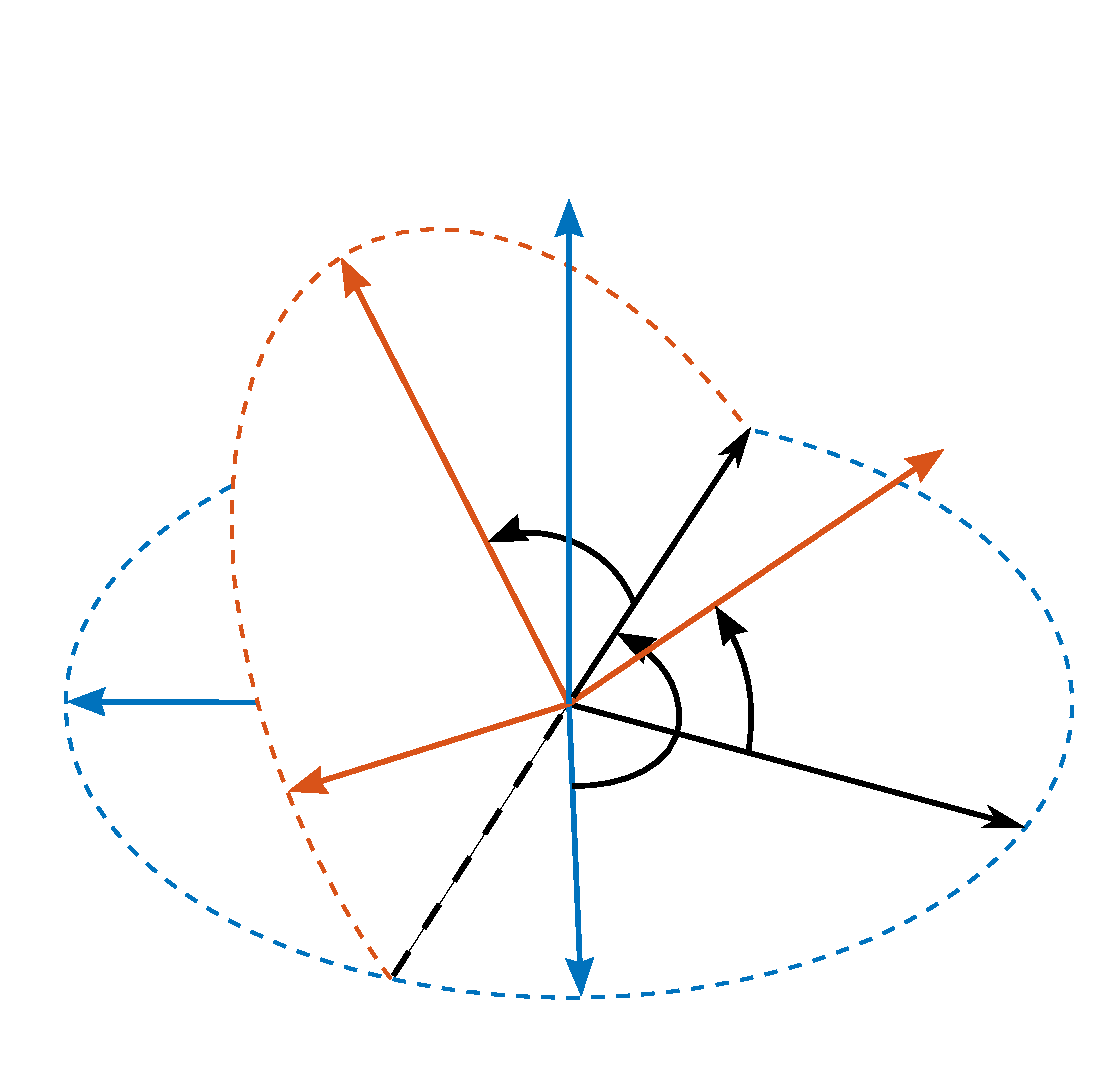
\includegraphics[width=.8\textwidth]{Figures/taitbryan.eps}};
    
\node [] at (0.5,0.2) {$\phi$};
\node [] at (0.65,-1.85) {$\psi$};
\node [] at (1.55,-0.9) {$\theta$};

\node [] at (-3.4,-1.1) {$x$};
\node [] at (0.25,-3.3) {$y$};
\node [] at (0.12,2.43) {$z$};

\node [] at (1.5,1) {$y'$};
\node [] at (3.4,-1.9) {$x'$};
\node [] at (2.8,0.6) {$X$};
\node [] at (-1.5,2.05) {$Y$};
\node [] at (-2.0,-1.7) {$Z$};
\end{tikzpicture}
\caption[Representation of the rotated body frame with respect to the world frame.]{Representation of the body frame, depicted in red, with respect to the world frame, depicted in blue \cite{Wiki_taitbryan}. The body frame was rotated by the Euler angles $\psi, \theta, \phi$ about the axes $z, y', X$, respectively.} \label{fig:Euler_angles}
\end{figure}

Euler angles are a simple and intuitive means to represent rotations in three-dimensional space. However, for the above mentioned parameterisation they have singularities at values of $\theta = n \pi$, $n \in \mathbb{Z}$. At these points a rotation about the $x$-axis and the $z$-axis constitute the same motion, which results in the loss of one degree of freedom and makes changes in $\phi$ and $\psi$ indistinguishable. This phenomenon is called \emph{gimbal lock}.

\subsection{Transformation Matrices}

Coordinates representing a point in one coordinate system can be transformed to another, given the angles between the two coordinate systems are known. Such a transformation can be expressed as a multiplication of a matrix with the coordinate vector that is to be transformed. Let $\bm{E}$ denote the orthonormal basis $\{x, y, z\} \in \mathbb{R}^3$ and let $\bm{E}'$ denote the orthonormal basis $\{X, Y, Z\} \in \mathbb{R}^3$. Furthermore, let $\bm{p}$ denote the position vector of an arbitrary point in three-dimensional Euclidean space, expressed in terms of $\bm{E}$. The coordinate transformation that maps $\bm{p}$ to its representation in $\bm{E}'$ is given by the linear transformation $\bm{\Omega}_{\bm{E} \rightarrow \bm{E}'}$,

\begin{equation}\label{eq:transformation}
\begin{split}
  \bm{\Omega}_{\bm{E} \rightarrow \bm{E}'}: \mathbb{R}^3 &\rightarrow \mathbb{R}^3 \\
  \bm{p} &\mapsto \bm{T}(\psi, \theta, \phi) \bm{p} \,,
\end{split}
\end{equation}

\noindent
where the \emph{transformation matrix} $\bm{T}$ is a function of the rotation angles $\psi, \theta, \phi$ between the coordinate axes.

In order to transform a coordinate vector from the world frame to the body frame, according to the common aerospace rotation sequence mentioned above, the transformation matrix $\bm{T}_{wb}$ is given by

\begin{equation}\label{eq:transformation_matrices}
\begin{split}
\bm{T}_{wb} & = \bm{T}_x(\phi) \bm{T}_y(\theta) \bm{T}_z(\psi) \\
 & = {\left[ \begin{smallmatrix}
    1 \; & 0 \; & 0 \\
    0 \; & \cos \phi \; & \sin \phi \\
    0 \; & -\sin \phi \; & \cos \phi
    \end{smallmatrix}\right]}
    {\bigg[ \begin{smallmatrix}
    \cos \theta \; & 0 \; & -\sin \theta \\
    0 \; & 1 \; & 0 \\
    \sin \theta \; & 0 \; & \cos \theta
    \end{smallmatrix} \bigg]}
    {\left[\begin{smallmatrix}
    \cos \psi \; & \sin \psi \; & 0 \\
    -\sin \psi \; & \cos \psi \; & 0 \\
    0 \; & 0 \; & 1
    \end{smallmatrix}\right]}\\
 & = {\left[\begin{smallmatrix}
   \cos \theta \cos \psi \; &
    \cos \theta \sin \psi \; &
   -\sin \theta \\
    \sin \phi \sin \theta \cos \psi - \cos \phi \sin \psi \;\; &
    \sin \phi \sin \theta \sin \psi + \cos \phi \cos \psi \;\; &
    \sin \phi \cos \theta \\
    \cos \phi \sin \theta \cos \psi + \sin \phi \sin \psi \;\; &
    \cos \phi \sin \theta \sin \psi - \sin \phi \cos \psi \;\; &
    \cos \phi \cos \theta
  \end{smallmatrix}\right]}
\end{split}\,.
\end{equation}

\noindent
Plugged in Equation \ref{eq:transformation}, the pre-multiplications of the matrices $\bm{T}_x(\phi)$, $\bm{T}_y(\theta)$, and $\bm{T}_z(\psi)$ to the vector $\bm{p}$ represent the coordinate rotations about the single axes $x, y', Z$, according to the right hand rule, respectively. That is, the function $\bm{\Omega}_{\bm{E} \rightarrow \bm{E}'}$ maps the vector $\bm{p}$ to its orthogonal projection onto the axes of the coordinate system that results from the respective two-dimensional rotation of $\phi, \theta, \psi$ about the axes $x, y', Z$. This is illustrated for a single rotation around the $z$-axis by an angle $\psi$ in Figure \ref{fig:transformation_matrix}. Note that $\{x', y', z'\}$ denotes the coordinate frame after the first elemental rotation. The matrices $\bm{T}_x(\phi), \bm{T}_y(\theta)$, and $\bm{T}_z(\psi)$ are also known as \emph{direction cosine matrices}, since their elements are the cosines of the unsigned angles between the body-fixed axes and the axes of the world frame, as shown in \cite{diebel2006attitude}. The Blender Game Engine \cite{blender} used for the simulations in Chapter \ref{ch:experiments} assumes a right-handed east-north-up coordinate system. Then, the matrix $\bm{T}_{bw}$ that transforms a coordinate vector from the body frame to the world frame is given by

\begin{figure}[t]
\centering

\tdplotsetmaincoords{60}{110}

\begin{tikzpicture}[scale=6,tdplot_main_coords]
\definecolor{mycolor1}{rgb}{0.00000,0.44701,0.74100}%
\definecolor{mycolor2}{rgb}{0.85000,0.32501,0.09801}%

\coordinate (O) at (0,0,0);
\pgfmathsetmacro{\psivec}{55}
\tdplotsetcoord{P}{0.8}{44}{\psivec}

\draw[thick,->] (0,0,0) -- (.8,0,0) node[anchor=north west]{$x$};
\draw[thick,->] (0,0,0) -- (0,.8,0) node[anchor=north west]{$y$};

\tdplotsetrotatedcoords{0}{0}{25}

\draw[thick,mycolor1,tdplot_rotated_coords,->] (0,0,0) -- (.8,0,0) node[anchor=north west]{$x'$};
\draw[thick,mycolor1,tdplot_rotated_coords,->] (0,0,0) -- (0,.8,0) node[anchor=west]{$y'$};
\draw[very thick,mycolor1,tdplot_rotated_coords] (0,0,0) -- (0, 0.25, 0) node[anchor=south east]{$p_y'$};
\draw[thick,mycolor1,tdplot_rotated_coords,->] (0,0,0) -- (0,0,.8) node[anchor=north west]{$z'=z$};
\draw[very thick,mycolor1,tdplot_rotated_coords] (0,0,0) -- (0.507, 0, 0) node[pos=0.9, label={left:$p_x'$}, rounded corners=1pt]{};
\draw[very thick,mycolor1,tdplot_rotated_coords] (0,0,0) -- (Pz) node[pos=0.5, label={left:$p_z'$}]{};

%draw a vector from origin to point (P) 
\draw[-stealth,color=mycolor2] (O) -- node [anchor=south]{$\bm{p}$}(P);

%draw projection on xy plane, and a connecting line
\draw[dashed, mycolor2] (O) -- (Pxy);
\draw[dashed, mycolor2] (P) -- (Pxy);
\draw[dashed] (Px) -- (Pxy);
\draw[dashed] (Py) -- (Pxy);

\tdplotdrawarc[-stealth]{(0,0,0)}{0.58}{0}{25}{anchor=north}{$\psi$}

\draw[dashed] (0.8,0,0) arc (0:115:0.8);

\draw[dashed, mycolor1, tdplot_rotated_coords] (0.507, 0, 0) -- (Pxy);
\draw[dashed, mycolor1, tdplot_rotated_coords] (0, 0.25, 0) -- (Pxy);
\draw[dashed, mycolor1, tdplot_rotated_coords] (P) -- (Pz);

\end{tikzpicture}
\caption[An exemplary coordinate rotation about the $z$-axis, illustrating the orthogonal projection on the resulting axes.]{An exemplary coordinate rotation about the $z$-axis by an angle $\psi$, illustrating the orthogonal projection $(p_x', p_y', p_z')$ of the position vector $\bm{p}$ on the resulting axes $x', y', z'$.}
	\label{fig:transformation_matrix}
\end{figure}


\begin{equation}\label{eq:cbw}
\bm{T}_{bw} = {\left[\begin{smallmatrix}
   \cos \theta \cos \psi \; &
    \sin \phi \sin \theta \cos \psi - \cos \phi \sin \psi \; &
    \cos \phi \sin \theta \cos \psi + \sin \phi \sin \psi \\
    \cos \theta \sin \psi \;\; &
    \sin \phi \sin \theta \sin \psi + \cos \phi \cos \psi \;\; &
    \cos \phi \sin \theta \sin \psi - \sin \phi \cos \psi \\
    -\sin \theta \;\; &
    \sin \phi \cos \theta \;\; &
    \cos \phi \cos \theta
  \end{smallmatrix}\right]}\,.
\end{equation}

\noindent
Note that $\bm{T}_{bw} = \bm{T}^T_{wb} = \bm{T}^{-1}_{wb}$. Thus, $\bm{T}^{ }_{bw}$ and $\bm{T}_{wb}$ are orthogonal matrices so that $\bm{T}^{ }_{bw} \bm{T}_{wb} = \bm{I}_3$, where $\bm{I}_3 \in \mathbb{R}^{3 \times 3}$ is the identity matrix. This makes sense as forward and backward rotations should not alter the vector $\bm{p}$.


\section{The Probabilistic State-space Model}\label{sec:prob_model}

In this section we will derive the state-space model for the particle filters, which is comprised of two components, i.\,e. the system model and the measurement model, in accordance with Equations \ref{eq:generic-state_dynamics} and \ref{eq:generic-measurement}.

\subsection{The System Model}\label{sec:system_model_prob}

The plant dynamics of a continuous-time system can be expressed as a set of $n_{\bm{x}}$ coupled first-order ordinary differential equations, known as the \emph{state equations} \cite{rowell2002state}, 

\begin{equation} \label{eq:state_vector_derivative}
  \dot{\bm{x}} = \bm{f}(\bm{x}, \bm{u}, t)\,,
\end{equation}

\noindent
where $\dot{\bm{x}}$ consists of the component-wise time derivatives of the state vector $\bm{x}$, expressed in terms of the state variables $x_1(t), \dots, x_{n_{\bm{x}}}(t)$, and the control inputs $u_1(t), \dots, u_{n_{\bm{u}}}(t)$. Explicitly, its elements are given by

\begin{equation}
  \dot{x}_i = f_i(\bm{x}, \bm{u}, t) = \frac{dx_i}{dt} \,, \quad i \in \{1, \dots, n_{\bm{x}}\}\,.
\end{equation}

\noindent
Given this state-space representation, the system state at any instant $t$ may be interpreted as a point in an $n_{\bm{x}}$-dimensional state space whose axes are the state variables. The dynamic state response $\bm{x}(t)$ can be interpreted as a trajectory traced out in the state space. 

\subsubsection{Discretisation of the State Equations}

Given a \emph{linear} \emph{time-invariant} system in state-space form, 

\begin{equation}\label{eq:linear_continuous}
  \dot{\bm{x}}(t) = \bm{A} \bm{x}(t) + \bm{G} \bm{u}(t)\,,
\end{equation}

\noindent
and its solution

\begin{equation}\label{eq:general_solution_system}
  \bm{x}(t) = e^{\bm{A}(t-t_0)} \bm{x}(t_0) +\int_{t_0}^t e^{\bm{A}(t - \tau)}\bm{G}\bm{u}(\tau)d\tau\,,
\end{equation}

%\begin{equation}\label{eq:general_solution_system}
%  \bm{x}(t) = \bm{\Phi}(t-t_0) \bm{x}(t_0) +\int_{t_0}^t \bm{\Phi}(t - \tau)\bm{G}(\tau)\bm{u}(\tau)d\tau\,,
%\end{equation}

\noindent
we shall discretise the continuous-time system using a discrete time index $k$, such that

\begin{equation}
  t = k T_s\,,
\end{equation}

\noindent
where $T_s$ is the sampling period. Our goal then is to determine a dynamical relation of the following form:

\begin{equation}\label{eq:discrete_plant_dynamics}
  \bm{x}_{k + 1} = \bm{\Phi} \bm{x}_k + \bm{B} \bm{u}_k, \quad k \in \{0, 1, 2, \dots\}\,,
\end{equation}

\noindent
where we replaced $\bm{x}(k T_s)$ by $\bm{x}_k$ and $\bm{u}(k T_s)$ by $\bm{u}_k$ for the sake of brevity.

In the following derivation of the matrices $\bm{\Phi}$ and $\bm{B}$, we assume the control input $\bm{u}(t)$ is constant over the sampling interval, such that the following holds:

\begin{equation}
  \bm{u}(t) = \bm{u}(k T_s), \quad kT_s \leq t < (k+1) T_s\,.
\end{equation}

\noindent
Setting $t_0 = kT_s$ and $t = (k+1) T_s$ in Equation \ref{eq:general_solution_system} yields

\begin{equation}\label{eq:general_solution_system_discrete}
  \bm{x}\big((k+1) T_s\big) = e^{\bm{A}T_s} \bm{x}(kT_s) +\int_{kT_s}^{(k+1) T_s} e^{\bm{A}\big[(k+1) T - \tau\big]}\bm{G}\bm{u}(\tau)d\tau\,.
\end{equation}

\noindent
Using that the control input is constant within the interval from $kT_s$ to $(k + 1)T_s$, as is the matrix $\bm{G}$, we can rewrite $\bm{x}\big((k+1) T_s\big)$ as

\begin{equation}\label{eq:general_solution_system_discrete}
  \bm{x}\big((k+1) T_s\big) = e^{\bm{A}T_s} \bm{x}(kT_s) +\int_{kT_s}^{(k+1) T_s} e^{\bm{A}\big[(k+1) T - \tau\big]}d\tau \bm{G}\bm{u}(k T_s)\,,
\end{equation}

\noindent
or shorter as

\begin{equation}\label{eq:general_solution_system_discrete}
  \bm{x}_{k+1} = e^{\bm{A}T_s} \bm{x}_k +\int_{kT_s}^{(k+1) T_s} e^{\bm{A}\big[(k+1) T - \tau\big]}d\tau \bm{G}\bm{u}_k\,.
\end{equation}

\noindent
Changing variables, such that $(k+1)T - \tau = \lambda$, yields

\begin{equation}\label{eq:general_solution_system_discrete}
  \bm{x}_{k+1} = e^{\bm{A}T_s} \bm{x}_k +\int_{0}^{T_s} e^{\bm{A}\lambda}d\lambda \bm{G}\bm{u}_k\,.
\end{equation}

\noindent
By comparison with Equation \ref{eq:discrete_plant_dynamics} we may now identify the matrices $\bm{\Phi}$ and $\bm{B}$ as

\begin{equation}
  \bm{\Phi} = e^{\bm{A}T_s}\,,
\end{equation}

\begin{equation}\label{eq:control_matrix_discrete}
  \bm{B} = \int_{0}^{T_s} e^{\bm{A}\lambda}d\lambda \bm{G}\,.
\end{equation}

In order to obtain the state transition matrix $\bm{\Phi}$, as outlined in \cite{zarchan2009fundamentals}, we can use a Taylor-series expansion of $e^{\bm{A}T_s}$,

\begin{equation}\label{eq:As}
\begin{split}
  \bm{\Phi} = e^{\bm{A}T_s} &= \sum_{n=0} ^ {\infty} \frac {\bm{A}^{n} T_s^n}{n!} \\
  &= \bm{I}_{n_{\bm{x}}} + \bm{A}T_s + \frac{\bm{A}^2 T_s^2}{2!} +\frac{\bm{A}^{3} T_s^3}{3!} + \dots\,,
\end{split}
\end{equation}
 
\noindent
where $\bm{I}_{n_{\bm{x}}} \in \mathbb{R}^{{n_{\bm{x}}} \times {n_{\bm{x}}}}$ is the identity matrix. Truncating the Taylor series after the first order terms yields the \emph{linear approximation} of the state transition matrix:

\begin{equation}\label{eq:state_transition_approx}
  \bm{\Phi} \approx \bm{I}_{n_{\bm{x}}} + \bm{A}T_s\,.
\end{equation}

\noindent
Using a Taylor series expansion of Equation \ref{eq:control_matrix_discrete} and integrating term-by-term, we may obtain $\bm{B}$ as

\begin{equation}\label{eq:Bs}
\begin{split}
\bm{B} &= \int_{0}^{T_s} e^{\bm{A}\lambda}d\lambda \bm{G} \\
   &= \int_{0}^{T_s} \bigg( \bm{I}_{n_{\bm{u}}} + \bm{A}\lambda + \frac{\bm{A}^2\lambda^2}{2!} +\frac{\bm{A}^3\lambda^3}{3!} + \cdots \bigg) d\lambda \bm{G} \\
   &= \Bigg( \int_{0}^{T_s}\bm{I}_{n_{\bm{u}}} d\lambda + \int_{0}^{T_s}\bm{A}\lambda d\lambda + \int_{0}^{T_s}\frac{\bm{A}^2\lambda^2}{2!} d\lambda + \int_{0}^{T_s}\frac{\bm{A}^3\lambda^3}{3!} d\lambda + \cdots \Bigg) \bm{G} \\
   &= \bm{G}T_s + \frac{\bm{A}\bm{G}T_s^2}{2!} + \frac{\bm{A}^2\bm{G}T_s^3}{3!} + \dots \,.
\end{split}
\end{equation}
 
 \noindent
 Again, taking the first term only, such that
 
 \begin{equation}
\bm{B} \approx \bm{G}T\,,
\end{equation}

\noindent
and plugging $\bm{B}$ together with $\bm{\Phi}$ of Equation \ref{eq:state_transition_approx} into Equation \ref{eq:discrete_plant_dynamics} yields Euler’s forward approximation:

\begin{equation}\label{eq:euler_approximation}
  \bm{x}_{k + 1} \approx (\bm{I}_{n_{\bm{x}}} + \bm{A}T_s) \bm{x}_k + \bm{G}\bm{u}_k T_s, \quad k \in \{0, 1, 2, \dots\}\,.
\end{equation}

\noindent
However, Equations \ref{eq:As} and \ref{eq:Bs} can easily be implemented in software. Therefore, terminating the series when the terms become smaller than some desired threshold provides arbitrarily precise results \cite{lewis1992applied}.


\subsubsection{Discretisation of the Modelled System}

The state vector of the robot is given by
 
\begin{equation} \label{eq:state_vector}
  \bm{x}_k = \begin{bmatrix}
  	x_k, & y_k, & z_k
  \end{bmatrix}^T \in \mathbb{R}^{n_{\bm{x}}=3}, \quad k \in \{0, 1, 2, \dots\}\,,
\end{equation}

\noindent
where its elements correspond to the coordinates describing the three-dimensional position $(x_k, y_k, z_k)$ of the robot at time step $k$, expressed in the world frame.
The plant dynamics of the modelled system are governed by the linear differential equation

\begin{equation} \label{eq:state_vector_derivative}
  \dot{\bm{x}} = \bm{A} \bm{x}(t) + \bm{G} \bm{u}(t) = \begin{bmatrix}
  v_x^{[w]}(t) \\
  v_y^{[w]}(t) \\ 
  v_z^{[w]}(t) \end{bmatrix}\,,
\end{equation}

\noindent
with the control input $\bm{u}(t) = \big[v_x^{[w]}(t), v_y^{[w]}(t), v_z^{[w]}(t)\big]^T$, whose components denote the nominal linear velocity in $x$, $y$, and $z$ direction, respectively, stated in terms of the world frame. Equating coefficients in Equation \ref{eq:state_vector_derivative} lets us identify the remaining variables as $\bm{A} = 0$ and $\bm{G} = \bm{I}_{n_{\bm{u}}}$. Plugging $\bm{A}$ and $\bm{G}$ into Equations \ref{eq:As} and \ref{eq:Bs} yields $\bm{\Phi} = \bm{I}_{n_{\bm{x}}}$ and $\bm{B} = \bm{I}_{n_{\bm{u}}} T_s$. Plugging now both $\bm{\Phi}$ and $\bm{B}$ into Equation \ref{eq:discrete_plant_dynamics}, we have

\begin{equation}
  \bm{x}_{k + 1} = \bm{x}_k + \bm{u}_k T_s, \quad k \in \{0, 1, 2, \dots\}\,.
\end{equation}

Since the robot's nominal linear velocity is naturally stated in terms of its body frame, as $\bm{u}^{[b]}_k = \big[v_{x, k}^{[b]}, v_{y, k}^{[b]}, v_{z, k}^{[b]}\big]^T$, it has to be transformed to the world frame according to Equation \ref{eq:transformation}, using the transformation matrix $\bm{T}_{bw}(\psi_k, \theta_k, \phi_k)$ of Equation \ref{eq:cbw},

\begin{equation}
  \bm{x}_{k + 1} = \bm{x}_k + \bm{T}_{bw}(\psi_k, \theta_k, \phi_k) \bm{u}^{[b]}_k T_s, \quad k \in \{0, 1, 2, \dots\}\,
\end{equation}

\noindent
Note that with the state equations at hand this is the best model available and a consequence of $\bm{A} = 0$. Although the form is similar, contrary to the claim in \cite{nicol2017}, this result is no Euler approximation but instead reflects the limited knowledge about the modelled system.
 
 Adhering to the notation used above, we subtract $1$ from each discrete time index $k$ and add noise terms to the individual variables, to take into account the inherent uncertainty in the model,

\begin{equation}\label{eq:system_model_euler}
\begin{split}
  \bm{x}_{k} &= \bm{\phi}_{k-1}(\bm{x}_{k-1}, \bm{u}_{k-1}, \bm{w}_{k-1}) \\
  &= \bm{x}_{k-1} + \bm{T}_{bw}\big(\psi_{k-1} + w_{\psi, {k-1}}, \theta_{k-1} + w_{\theta,{k-1}}, \phi_{k-1} + w_{\phi,{k-1}}\big) \\
  &\mathrel{\phantom{= \bm{x}_{k-1}}}\: \cdot \: \big(\bm{u}^{[b]}_{k-1} + \bm{w}_{v, {k-1}}\big) T_s, \quad k \in \{1, 2, 3, \dots\}\,.
  \end{split}
\end{equation}

\noindent
The process noise vector $\bm{w}_k = \big[\bm{w}_{v,k}, \bm{w}_{{\mathrm{Eul}},k}\big] \in \mathbb{R}^{n_{\bm{w}}=6}$, with $\bm{w}_{{\mathrm{Eul}},k} = \big[w_{\psi, {k}}, w_{\theta, {k}}, w_{\phi, {k}}\big]^T$ and $\bm{w}_{v,k} = \big[w_{v_x, {k}}, w_{v_y, {k}}, w_{v_z, {k}}\big]^T$, is assumed to be normally distributed with zero mean and constant covariance matrix $\bm{Q}_k \in \mathbb{R}^{n_{\bm{w}} \times n_{\bm{w}}}$, given by

\begin{equation}
\bm{Q}_k = \begin{bmatrix}
  \sigma^2_{\bm{v}} & 0 & 0 & 0 & 0 & 0 \\
  0 & \sigma^2_{\bm{v}} & 0 & 0 & 0 & 0 \\
  0 & 0 & \sigma^2_{\bm{v}} & 0 & 0 & 0 \\
  0 & 0 & 0 & \sigma^2_{\mathrm{Eul}} & 0 & 0 \\
  0 & 0 & 0 & 0 & \sigma^2_{\mathrm{Eul}} & 0 \\
  0 & 0 & 0 & 0 & 0 & \sigma^2_{\mathrm{Eul}} \\
\end{bmatrix}, \quad k \in \{0, 1, 2, \dots\}\,.
\end{equation}

\noindent
Due to the relation $\operatorname{Cov}(w_i,w_i) = \operatorname{Var}(w_i)$, the diagonal elements represent the respective variances of the elements $w_1, \dots, w_n$ of the process noise vector $\bm{w}$. The other elements are the covariances of all possible pairs of the random variables of the process noise vector. The noise processes interfering with the individual Euler angles and the velocity inputs, respectively, are modelled as uncorrelated so that the remaining elements of $\bm{Q}_k$ are zero.

With the process model of Equation \ref{eq:system_model_euler} at hand, we can now state the transition prior probability distribution, which is employed in the computation of the importance weights of the unscented particle filter, as a Gaussian with mean $\bm{x}_k - \bm{\phi}_{k-1}(\bm{x}_{k-1}, \bm{u}_{k-1}, \bm{0})$ and covariance $\bm{Q}_k$,

\begin{equation}
p(\bm{x}_k\,|\,\bm{x}_{k-1}, \bm{u}_{k-1}) = \mathcal{N}\big(\bm{x}_k - \bm{\phi}_{k-1}(\bm{x}_{k-1}, \bm{u}_{k-1}, \bm{0}), \bm{Q}_k \big)\,.
\end{equation}

\subsection{The Measurement Model}\label{sec:measurement_model_prob}

Provided the position of $n_{\bm{z}}$ landmarks is known, theoretically the position of the robot can be computed from the distances between the robot and multiple landmarks using lateration. Considering the distance between the robot and one landmark alone, possible positions the robot may have are situated on a sphere around the landmark, with its radius equal to the distance to the robot. In order to unambiguously determine the exact position in three-dimensional space four landmarks are required. Then, their surrounding spheres with the respective radii $d_i$ ideally intersect in one point identical with the robot's position. Mathematically, lateration can be expressed as finding the solution of the following system of quadratic equations:


\begin{equation}\label{eq:lateration}
  (x - x_i)^2 + (y-y_i)^2 + (z - z_i)^2 = d_i^2, \quad i \in \{1, \dots, n_{\bm{z}}\}\,,
\end{equation}

\noindent
where $(x, y, z)$ are the coordinates of the robot and $(x_i, y_i, z_i)$ are the known coordinates of the $i$-th of $n_{\bm{z}}$ landmarks in three-dimensional space, respectively. For the sake of clarity of presentation, Figure \ref{fig:trilateration} depicts exemplary the scenario for the determination of the two-dimensional position $(x, y)$ of a robot and the known positions $(x_i, y_i)$ of the landmarks $i \in \{1, 2, 3\}$.

\begin{figure}[t]
\centering
\begin{tikzpicture}[scale=1.0, auto, thick, node distance=3cm,>=latex']
    \pgftext{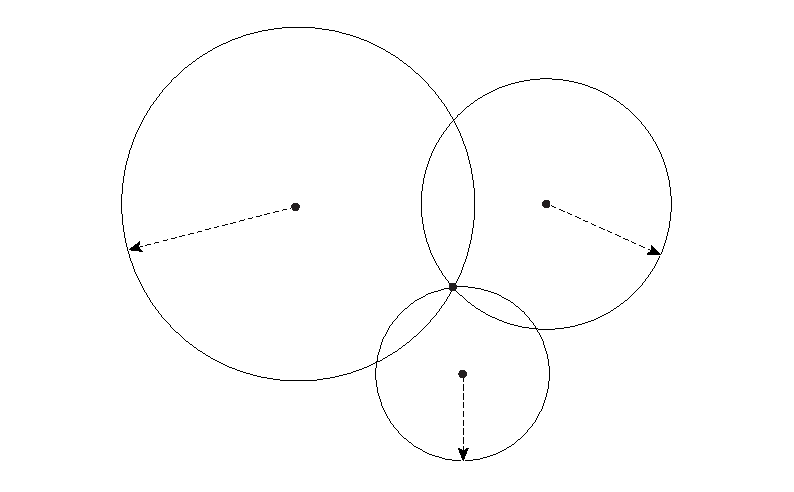
\includegraphics[width=1\textwidth]{Figures/trilateration}} at (0, 0);
    
    \node [] (a) at (2.3, 1.1) {$(x_2, y_2)$};
    \node [] (a) at (3, -0.1) {$d_2$};
     \node [] (a) at (-1.5, 1.1) {$(x_1, y_1)$};
     \node [] (a) at (-2.5, -0.1) {$d_1$};
     \node [] (a) at (1.7, -0.3) {$(x, y)$};
     \node [] (a) at (1.1, -1.6) {$(x_3, y_3)$};
     \node [] (a) at (1.4, -2.5) {$d_3$};
        
\end{tikzpicture}
\caption[Determination of the two-dimensional position of a robot given the known positions of three landmarks.]{Trilateration: depicted is the determination of the two-dimensional position $(x, y)$ of a robot from the distances $d_i$ to the three landmarks $i \in \{1, 2, 3\}$ with known positions $(x_i, y_i)$.}
	\label{fig:trilateration}
\end{figure}

Due to measurement noise, the radii morph into concentric spheres around the respective landmarks, so that there is not a precise intersection point anymore and simply solving a system of quadratic equations is not sufficient to determine the robot's position. Incorporating the uncertainty into the model using the noise term $\bm{v}_k $ yields the measurement vector $\bm{z}_k \in \mathbb{R}^{n_{\bm{z}}}$ of the modelled system as

\begin{equation} \label{eq:measurement_vector}
  \bm{z}_k = \begin{bmatrix} d_{1,k} \\ d_{2,k} \\ \vdots \\ d_{n_{\bm{z}},k} \end{bmatrix} = \begin{bmatrix}
  	\sqrt{(x_k - x_{1})^2 + (y_k - y_{1})^2 + (z_k - z_{1})^2} \\
  	\sqrt{(x_k - x_{2})^2 + (y_k - y_{2})^2 + (z_k - z_{2})^2} \\
  	\vdots \\
  	\sqrt{(x_k - x_{n_{\bm{z}}})^2 + (y_k - y_{n_{\bm{z}}})^2 + (z_k - z_{n_{\bm{z}}})^2}
  \end{bmatrix} + \bm{v}_k 
  \,,
\end{equation}

\noindent
where the $d_i$-s represent the distance between the robot and the $i$-th of $n_{\bm{z}}$ landmarks and the measurement noise process $\bm{v}_k \in \mathbb{R}^{n_{\bm{v}}}$ is modelled as zero-mean Gaussian white noise. The length $n_{\bm{z}}$ of the measurement vector is determined by the number of landmarks and is kept variable intentionally for experiments with different numbers of landmarks. The constant measurement noise covariance matrix $\bm{R}_k \in \mathbb{R}^{n_{\bm{v}} \times n_{\bm{v}}}$ is given by

\begin{equation}
\bm{R}_k = \begin{bmatrix}
  \sigma^2_{d} & 0 & 0 & 0\\
  0 & \sigma^2_{d} & 0 & 0\\
  \vdots &   & \ddots & \vdots\\
  0 & 0 & 0 & \sigma^2_{d}
\end{bmatrix}\,.
\end{equation}

\noindent
With the measurement model of Equation \ref{eq:measurement_vector} at hand, we can now state the likelihood function to be a Gaussian with mean $\bm{z}_k - \bm{h}_{k}(\bm{x}_{k}, \bm{0})$ and covariance $\bm{R}_k$,

\begin{equation}
p(\bm{z}_k\,|\,\bm{x}_{k}) = \mathcal{N}\big(\bm{z}_k - \bm{h}_{k}(\bm{x}_{k}, \bm{0}), \bm{R}_k \big)\,.
\end{equation}



\section{The Bounded-error Model}\label{sec: bounded_error}

In bounded-error state estimation, all model and measurement errors are assumed to vary around a central value within certain bounds \cite{Seignez2008ComplexitySO}. Only when the bounds are chosen conservatively enough, the estimation result may be trusted. Under real-life conditions, however, the measurement error is usually  normally distributed and therefore inherently unbound. The probability that a normal deviate $x$, with mean $\mu$ and standard deviation $\sigma$, lies in the range between $\mu - \xi \sigma$ and $\mu + \xi \sigma$, with $\xi \in \mathbb{R}^{+}$, can be computed using the Gauss error function as

\begin{equation} \label{eq:confidence}
 \operatorname{Pr}\big((x > \mu - \xi \sigma) \wedge (x < \mu + \xi \sigma)\big) = \operatorname{erf}\Bigg(\frac{\xi}{\sqrt{2}}\Bigg) = \frac{1}{\sqrt\pi}\int_{-\frac{\xi}{\sqrt{2}}}^{\frac{\xi}{\sqrt{2}}} e^{-t^2} \,dt \,.
\end{equation}

\noindent
To obtain a desired confidence interval, we inflate the real quantity $x$ to an interval $[x]$ as follows:

\begin{equation} \label{eq:state_vector_interval}
  [x] = [x - \xi \sigma,x + \xi \sigma\big] \,.
\end{equation}

\noindent
For $\xi = 3$ this leads to a probability that the interval covers a sample from the above mentioned Gaussian distribution of $99.73$ percent.

\subsection{The System Model}

The robot's interval state vector $[\bm{x}_k] \in [\mathbb{R}]^{n_{\bm{x}} = 3}$ is given by

\begin{equation} \label{eq:state_vector_interval}
  [\bm{x}_k] = \begin{bmatrix}
  	\big[\underline{x}_k, \overline{x}_k\big], & \big[\underline{y}_k, \overline{y}_k\big], & \big[\underline{z}_k, \overline{z}_k\big]
  \end{bmatrix}^T, \quad k \in \{0, 1, 2, \dots\}\,.
\end{equation}

\noindent
To predict the interval position $[\bm{x}_k]$, given the previous interval position $[\bm{x}_{k-1}]$, it requires an inclusion function $[\bm{\phi}_{k}]: [\mathbb{R}]^{n_{\bm{x}}} \rightarrow [\mathbb{R}]^{n_{\bm{x}}}$ of the state transition function $\bm{\phi}_{k}$. A straightforward way to obtain an inclusion function is replacing each expression in the system model given by Equation \ref{eq:system_model_euler} by its natural interval extension. Then we have

\begin{equation}\label{eq:system_model_int}
\begin{split}
  [\bm{x}_{k}] &= [\bm{\phi}_{k-1}]\big([\bm{x}_{k-1}], [\bm{u}_{k-1}], [\bm{w}_{k-1}]\big) = [\bm{x}_{k-1}] \\
  &\mathrel{\phantom{i}}+ [\bm{T}_{bw}]\big([\psi_{k-1}] + [w_{\psi,{k-1}}], [\theta_{k-1}] + [w_{\theta,{k-1}}], [\phi_{k-1}] + [w_{\phi,{k-1}}]\big) \\
  &\mathrel{\phantom{iiiiii}}\: \cdot \: \big([\bm{u}^{[b]}_{k-1}] + [\bm{w}_{v, {k-1}}]\big) T_s, \quad k \in \{1, 2, 3, \dots\}\,,
  \end{split}
\end{equation}

\noindent
where $[\bm{T}_{bw}]$ denotes the natural interval extension of the transformation matrix $\bm{T}_{bw}$ of Equation \ref{eq:cbw}.


\subsection{The Measurement Model}

Extending Equation \ref{eq:lateration} to intervals as follows, with $\bm{v}_{k} = 0$, yields the bounded-error measurement model $[\bm{h}_k]: [\mathbb{R}]^{n_{\bm{x}}} \rightarrow [\mathbb{R}]^{n_{\bm{z}}}$, which is used to construct the set $\mathbb{C}_k$ of $n_{\bm{z}}$ constraints of the form

\begin{equation} \label{eq:constraints}
\begin{split}
  [\bm{z}_k] &= \begin{bmatrix}
  	\big[d_{1,k} - \xi \sigma_{d}, d_{1,k} + \xi \sigma_{d}\big] \\
  	\big[d_{2,k} - \xi \sigma_{d}, d_{2,k} + \xi \sigma_{d}\big] \\
  	\vdots \\
  	\big[d_{n_{\bm{z}},k} - \xi \sigma_{d}, d_{n_{\bm{z}},k} + \xi \sigma_{d}\big]
  \end{bmatrix} \\
  &= [\bm{h}_k]\big([\bm{x}_k], 0 \big)\\
  &= \begin{bmatrix}
  	\sqrt{([x_k] - x_{1})^2 + ([y_k] - y_{1})^2 + ([z_k] - z_{1})^2} \\
  	\sqrt{([x_k] - x_{2})^2 + ([y_k] - y_{2})^2 + ([z_k] - z_{2})^2} \\
  	\vdots \\
  	\sqrt{([x_k] - x_{n_{\bm{z}}})^2 + ([y_k] - y_{n_{\bm{z}}})^2 + ([z_k] - z_{n_{\bm{z}}})^2}
  \end{bmatrix}\,.
  \end{split}
\end{equation}

\noindent
This model is motivated by the following notion. Given a noisy measurement $\bm{z}_k$ the true distance lies in the interval $[\bm{z}_k]$, with a probability that can be determined by Equations \ref{eq:confidence}. The concentric spheres described by the above constraints will overlap in certain regions of the search space. The region that is confined by the respective inner and outer sphere satisfies all the constraints and thus contains feasible robot positions. On the other hand, any point that lies outside does not satisfy the constraints and is therefore no solution. 

\section{Constrained Particle Filters}\label{sec: constraint-filters}

The above Bayesian filtering techniques have been developed for unconstrained conditions, which means that essentially any estimate in the state space is a possible solution to the filtering problem. However, in practical applications additional information about a process in the form of constraints are commonly encountered \cite{SHAO2010143}. These constraints may stem from physical laws, model restrictions or technological limitations \cite{chiang2002constrained}. Taking into account such important supplementary information about the state may improve the state estimation performance \cite{straka2012truncation}. The aim of constrained Bayesian filtering then is to find an estimate of the posterior probability distribution $p_C(\bm{x}_k\,|\,\bm{Z}_{k}, \bm{U}_{k-1})$ subject to the constraints,

\begin{equation}\label{eq:constraint_pdf}
\begin{split}
p_C(\bm{x}_k\,|\,\bm{Z}_{k}, \bm{U}_{k-1}) &= p(\bm{x}_k\,|\,\bm{Z}_{k}, \bm{U}_{k-1}, \bm{x}_{k} \in \bm{\mathbb{S}}_k) \\
  &= \begin{cases}
  	\zeta_k^{-1} p(\bm{x}_k\,|\,\bm{Z}_{k}, \bm{U}_{k-1}) & \quad \mathrm{if}\:\bm{x}_{k} \in \bm{\mathbb{S}}_k \\
  	0 & \quad \mathrm{otherwise}
  \end{cases}\,,
\end{split}
\end{equation}

\noindent
with the normalising constant

\begin{equation}
  \zeta_k = \operatorname{Pr}(\bm{x}_{k} \in \bm{\mathbb{S}}_k\,|\,\bm{Z}_{k}, \bm{U}_{k-1}) = \int_{\bm{\mathbb{S}}_k} p(\bm{x}_k\,|\,\bm{Z}_{k}, \bm{U}_{k-1}) d \bm{x}_{k}
\end{equation}

\noindent
and the set $\bm{\mathbb{S}}_k$ of states satisfying the constraints, according to Equation \ref{eq:solution_set}.

\subsection{Clipping}

A very simple approach to satisfy linear constraints is \emph{clipping}, which denotes mapping a point estimate lying outside the constrained region into it or project it right onto the boundary \cite{simon2006optimal}. We will use clipping for all six filters used for the experiments described in the next chapter. That is, whenever a particle or a sigma point lies outside the map, which is assumed to have linear boundaries parallel to one of the three axes of the world coordinate system, it is projected onto the boundary. Especially the covariance estimate of the unscented Kalman filter is positively influenced by mapping the sigma points instead of the estimate itself \cite{KANDEPU2008753}. In our estimation scenario, the clipping approach reflects a plausibility assessment of the environment. For instance, given a map as for the experiments below that assumes a position in $z$-direction of $0$ metres to be the sea surface, the underwater robot cannot be located above it, so that $z \leq 0$ holds for every position estimate. 



\subsection{Non-linear Constraints}

When dealing with multiple non-linear interval constraints according to Equation \ref{eq:constraints}, the projection on the boundary may not be straightforward in practice. Instead, one may simply discard particles outside the constrained regions and thereby trim the conditional probability distribution of the state with respect to the constraints, whilst preserving the shape of the PDF within the boundaries \cite{lang2007bayesian}. This method has moderate computational demands and generally leads to an improvement of the estimation accuracy \cite{teixeira2010unscented}. Modifying the generic particle filter so that it discards particles that violate constraints, we adopt the acceptance-rejection scheme in \cite{shao2010constrained},

\begin{equation}\label{eq:weights_new_particle}
   w^{(i)}_k = L^{(i)}_k\big(\hat{\bm{x}}^{(i)}_k\big) w^{(i)}_{k-1} \frac{p\big(\bm{z}_k\,|\,\hat{\bm{x}}^{(i)}_k\big) p\big(\hat{\bm{x}}^{(i)}_k\,|\,\bm{x}^{(i)}_{k-1}, \bm{u}_{k-1}\big)}{\pi\big(\hat{\bm{x}}^{(i)}_k\,|\,\bm{X}^{(i)}_{k-1}, \bm{Z}_{k}, \bm{U}_{k-1}\big)}, \quad i \in \{1, \dots, N\}\,,
\end{equation}

\noindent
with

\begin{equation}\label{eq:truncation_factor}
   L^{(i)}_k\big(\hat{\bm{x}}^{(i)}_k\big) = \begin{cases}
   	1 & \quad \mathrm{if}\:\hat{\bm{x}}^{(i)}_k \in \bm{\mathbb{S}}_k \\
   	0 & \quad \mathrm{otherwise}
   \end{cases}\,
\end{equation}

\noindent
Hence, the particles with zero weight will die out while resampling.


\section{The New Localisation Algorithms}\label{sec:new_filters}

We shall now describe the four newly proposed filter algorithms, all of which share the following features. The initial search space $[\bm{x}_0] \in [\mathbb{R}]^{n_{\bm{x}}}$ encompasses the entire map. The sequence of the $n_s$ control inputs and measurements is denoted by $\bm{U}_{n_s}$ and $\bm{Z}_{n_s}$, respectively. The probabilistic system model $\bm{\phi}_k: \mathbb{R}^{n_{\bm{x}}} \rightarrow \mathbb{R}^{n_{\bm{x}}}$ as well as the bounded-error system model $[\bm{\phi}_k]: [\mathbb{R}]^{n_{\bm{x}}} \rightarrow [\mathbb{R}]^{n_{\bm{x}}}$ and measurement model $[\bm{h}_k]: [\mathbb{R}]^{n_{\bm{x}}} \rightarrow [\mathbb{R}]^{n_{\bm{z}}}$ are assumed to be constant, therefore we can omit the index $k$. 


\subsection{Initialisation}\label{sec:filter_initialisation}

A robot solving the wake-up robot problem, by definition, does not know where it is and is aware of this fact. Thus, in the beginning of conventional Monte Carlo localisation using a bootstrap filter or an unscented particle filter, hypotheses of the robot's position are spread over the entire map. However, when additional information that confines the initial search space is available it may be used to restrict the spreading of particles to regions that  potentially contain the robot's true position and therefore increase the localisation accuracy.

A possible way of generating particles in the first iteration is to check whether a particle is inside a box or subpaving obtained by means of interval analysis and replacing it in case it is outside \cite{MACHADOCOELHO2017405, neulandh_ybridazation, neuland_set_inversion}. This may take a long time depending on the shape of the subpaving. A more efficient approach is uniformly generating particles inside the hull of a subpaving and killing the ones that are inconsistent with the constraints used for the bounded-error localisation by setting their importance weights to zero \cite{SHAO2010143}. 

\begin{figure}
	\centering
	\setlength\figureheight{0.7\textwidth} 	
	\setlength\figurewidth{0.9\textwidth}		
	\tikzsetnextfilename{sivia3d_real}		
	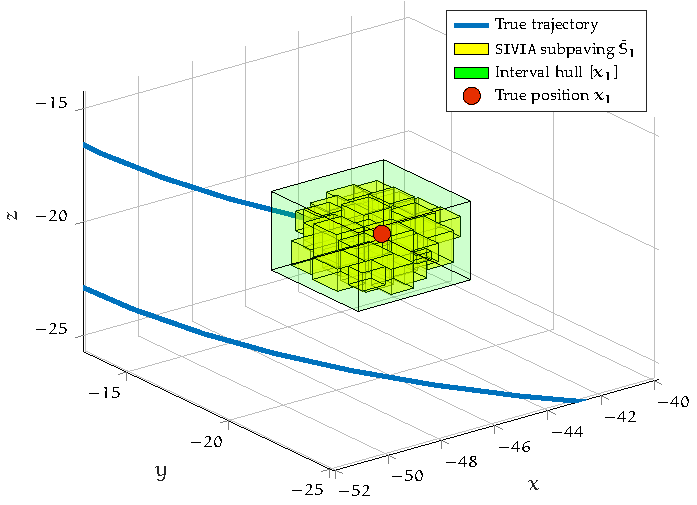
\includegraphics[width=\textwidth]{Tikz/sivia3d_real.tikz}		
	\caption[The result of the \texttt{SIVIA} algorithm in three dimensions for an exemplary trajectory.]{The result of the \texttt{SIVIA} algorithm in three dimensions for an exemplary trajectory and $\epsilon = 1.5\,$m depicted in yellow and its interval hull depicted in green.}		
	\label{fig:sivia3d_real}			
\end{figure}


\begin{figure}
	\centering
	\setlength\figureheight{0.7\textwidth} 	
	\setlength\figurewidth{0.9\textwidth}		
	\tikzsetnextfilename{sivia_particles}		
	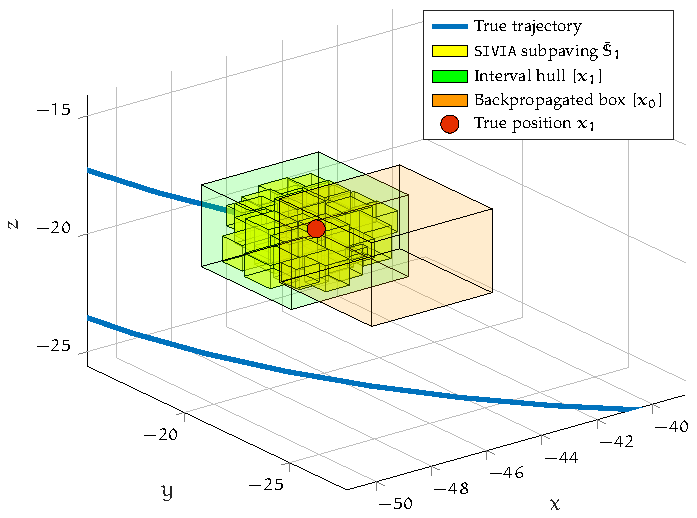
\includegraphics[width=\textwidth]{Tikz/sivia_particles.tikz}	
	\caption[Backpropagated box in relation to the interval hull of a \texttt{SIVIA} subpaving.]{Backpropagated box $[\bm{x}_0]$ in relation to the interval hull $[\bm{x}_1]$ of the \texttt{SIVIA} subpaving $\bar{\mathbb{S}}_1$.}			
	\label{fig:sivia_particles}			
\end{figure}


\begin{figure}
	\centering
	\setlength\figureheight{0.7\textwidth} 	
	\setlength\figurewidth{0.9\textwidth}		
	\tikzsetnextfilename{initial_particles}		
	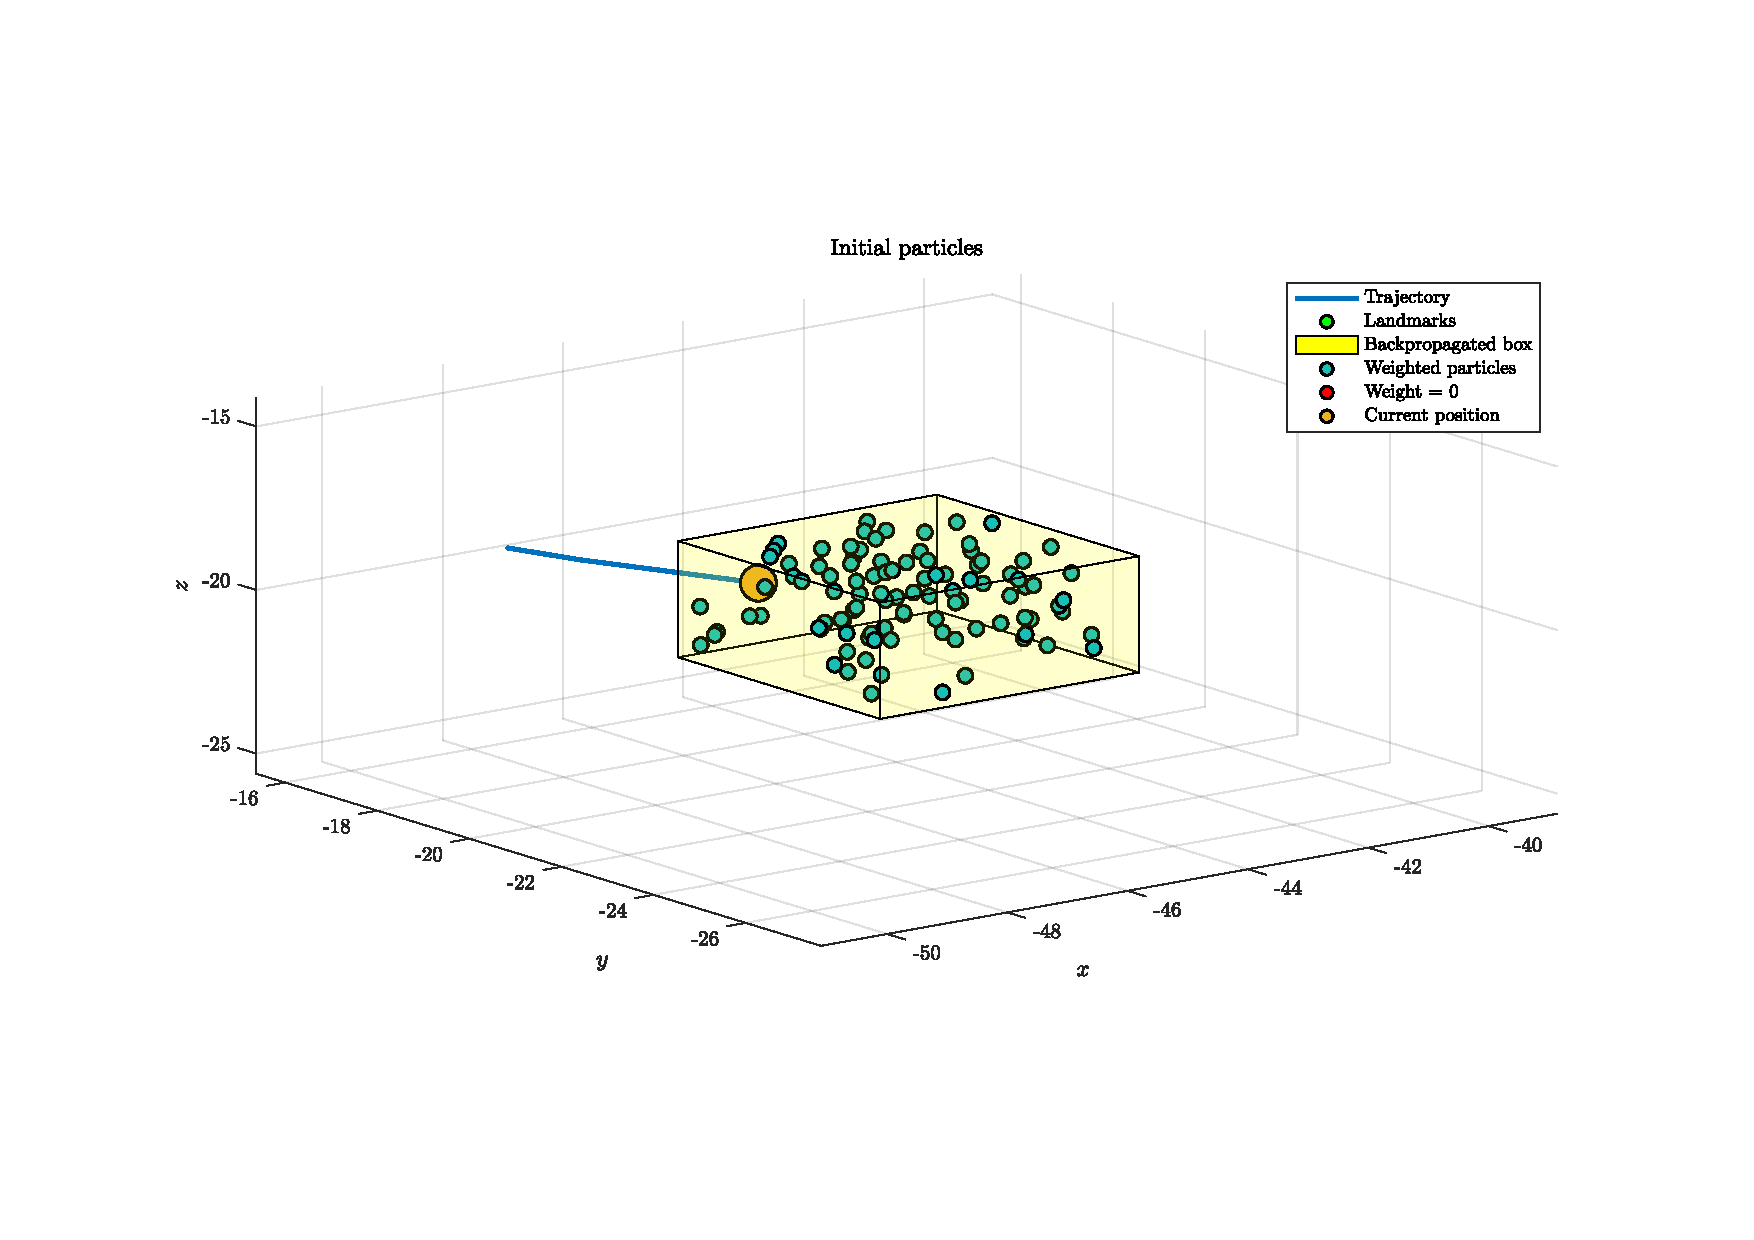
\includegraphics[width=\textwidth]{Tikz/initial_particles.tikz}	
	\caption[Uniformly spread initial particles in a backpropagated box.]{Uniformly spread initial particles in the backpropagated box $[\bm{x}_0]$.}		
	\label{fig:initial_particles}			
\end{figure}




The bounded-error measurement model $[\bm{h}]$ can be used to construct a set $\mathbb{C}_k$ of $n_{\bm{z}}$ constraints that are used to narrow down the search space by means of a contractor or by means of \texttt{SIVIA}. Since the first measurement, per definition of the Bayesian filter, only comes available at time step $k = 1$, this measurement and its associated constraints are used to contract the search space or obtain a subpaving $\bar{\mathbb{S}}_1$ that approximates the solution set $\mathbb{S}_1$, respectively. Figure \ref{fig:sivia3d_real} shows the result of the \texttt{SIVIA} algorithm in three dimensions with respect to an exemplary trajectory and $\epsilon = 1.5\,$m as well as its interval hull. Then, the respective contracted box or interval hull of the subpaving, both denoted by $[\bm{x}_{1}]$, are propagated backwards by one time step. Rearranging Equation \ref{eq:system_model_int}, we have

\begin{equation}\label{eq:system_model_int_back}
\begin{split}
  [\bm{x}&_{k-1}] = [\bm{x}_{k}] \\
  &- [\bm{T}_{bw}]\big([\psi_{k-1}] + [w_{\psi,{k-1}}], [\theta_{k-1}] + [w_{\theta,{k-1}}], [\phi_{k-1}] + [w_{\phi,{k-1}}]\big) \\
  &\mathrel{\phantom{iiii}}\: \cdot \: \big([\bm{u}^{[b]}_{k-1}] + [\bm{w}_{v, {k-1}}]\big) T_s, \quad k \in \{1, 2, 3, \dots\}\,.
  \end{split}
\end{equation}

\noindent
Plugging in $[\bm{x}_{1}]$ and the zeroth control input, that is $[\bm{u}^{[b]}_{k-1}] = \bm{u}^{[b]}_{0}$, results in the box $[\bm{x}_0]$, which is depicted in Figure \ref{fig:sivia_particles}. This box confines the uniform spreading of equally weighted particles drawn from $p(\bm{x}_0)$, which constitute the set $\big\{\big(\bm{x}^{(i)}_{0}, N^{-1}\big)\big\}_{i=1}^N$ as depicted in Figure \ref{fig:initial_particles}. Given this initial distribution, in principle, any standard Bayesian filter algorithm could be applied.
 
\subsection{Detection of Kidnapping}

Previous hybrid methods based on Monte Carlo simulation and interval analysis maintain the respective contracted box \cite{neulandh_ybridazation} or subpaving \cite{neuland_set_inversion} throughout the whole estimation process. Each particle that does not satisfy the constraints is replaced by a particle sampled from a uniform distribution that is confined by the respective bounded-error estimate or its interval hull. However, instead of generating new particles at every time step, the ones that are inconsistent with the constraints can be killed and the remaining ones can be reproduced while resampling. When all particles have zero weight, that is none of them satisfy all constraints, there has been a localisation failure. In other words, the robot has been kidnapped. Then, for the robot a reasonable action is to perform global localisation over the whole map. Therefore, the same steps as during the initialisation described in the previous section are carried out but using the current measurement instead of the first one. Carrying out a contraction of the search space or generating a \texttt{SIVIA} subpaving only in the very first iteration and in the iteration just after kidnapping, respectively, immensely reduces computational cost while preserving the benefits of bounded-error state estimation.


\begin{algorithm*}[t]
\caption[Particle filter with \texttt{HC4} contractor (\texttt{PFC})]{\texttt{PFC} (bootstrap particle filter with \texttt{HC4} contractor)}
\label{alg: pfc}
\begin{algorithmic}[1]
\Require $[\bm{x}_0], \quad \bm{U}_{n_s}, \quad \bm{Y}_{n_s}, \quad \bm{\phi}, \quad [\bm{\phi}], \quad [\bm{h}], \quad \xi > 0$ 
\Ensure $\big\{\hat{\bm{x}}_k\big\}, \quad \big\{\bm{P}_k\big\}, \quad k \in \{1, \dots, n\}$
\Statex
\Function{PFC}{$[\bm{x}_0], \bm{U}_{n_s}, \bm{Y}_{n_s}, \bm{\phi}, [\bm{\phi}], [\bm{h}], \xi$}
\For{$k \gets 1, n_s$}
\State $\mathbb{C}_k \gets$ \Call{constructConstraints}{$[\bm{h}], \bm{z}_{k}, \xi$} \Comment{Eq. \ref{eq:constraints}}
\If{$k = 1$} \Comment{initialise filter}
	\State $[\bm{x}_{k}] \gets$ \Call{contract}{$[\bm{x}_0], \mathbb{C}_k$} \label{marker} \Comment{contract using \texttt{HC4}}
	\State $[\bm{x}_{k-1}] \gets$ \Call{propagateBackwards}{$[\bm{x}_k]$} \Comment{Eq. \ref{eq:system_model_int_back}}
    \State $\mathbb{P}_{k-1} \gets$ \Call{drawParticles}{$N, [\bm{x}_{k-1}]$} \Comment{Eq. \ref{eq:draw_initial_particles}}
 \EndIf
 \State $\mathbb{P}_{k} \gets$ \Call{propagateParticles}{$\mathbb{P}_{k-1}$} \Comment{Eq. \ref{eq:propagate_particles}}
 \State $\mathbb{W}_{k} \gets$ \Call{weightParticles}{$\mathbb{P}_{k}, \mathbb{C}$} \Comment{Eq. \ref{eq:weights_new_particle}}
 \If{$\sum_{W \in \mathbb{W}_{k}}W = 0$} \Comment{restart localisation process}
 \State \Goto{marker}
 \EndIf
 \State $\mathbb{P}_{k} \gets$ \Call{resample}{$\mathbb{P}_{k}, \mathbb{W}_{k}$} \Comment{Eq. \ref{eq:resampling}}
 \State $\hat{\bm{x}}_k \gets$ \Call{mean}{$\mathbb{P}_{k}$} \Comment{Eq. \ref{eq:empirical_mean}}
 \State $\bm{P}_k \gets$ \Call{covariance}{$\hat{\bm{x}}_k, \mathbb{P}_{k}$} \Comment{Eq. \ref{eq:empirical_cov}}
\EndFor
\State \Return $\Big(\big\{\hat{\bm{x}}_k\big\}, \big\{\bm{P}_k\big\}\Big)$ 
\EndFunction
\end{algorithmic}
\end{algorithm*}



\subsection{Particle Filters with \texttt{HC4} Contractor}

Algorithm \ref{alg: pfc} depicts the particle filter with contractor (\texttt{PFC}). Initially, after the construction of the constraints, the search space is contracted using the \texttt{HC4} algorithm. The resulting box is propagated backwards by one time step and particles are spread uniformly within the box. These particles are propagated by the system model and weighted. Given there are non-zero weights, resampling is carried out and the empirical particle mean and covariance is returned. Otherwise, when all weights are zero, the localisation process is restarted by going to line 5. The filter loop is repeated for each of the $n_s$ samples.

\begin{algorithm*}[t]
\caption[Unscented particle filter with \texttt{HC4} contractor (\texttt{UPFC})]{\texttt{UPFC} (unscented particle filter with \texttt{HC4} contractor)}
\label{alg: upfc}
\begin{algorithmic}[1]
\Require $[\bm{x}_0], \quad \bm{U}_{n_s}, \quad \bm{Y}_{n_s}, \quad \bm{\phi}, \quad [\bm{\phi}], \quad [\bm{h}], \quad \xi > 0$ 
\Ensure $\big\{\hat{\bm{x}}_k\big\}, \quad \big\{\bm{P}_k\big\}, \quad k \in \{1, \dots, n\}$
\Statex
\Function{UPFC}{$[\bm{x}_0], \bm{U}_{n_s}, \bm{Y}_{n_s}, \bm{\phi}, [\bm{\phi}], [\bm{h}], \xi$}
\For{$k \gets 1, n_s$}
\State $\mathbb{C}_k \gets$ \Call{constructConstraints}{$[\bm{h}], \bm{z}_{k}, \xi$} \Comment{Eq. \ref{eq:constraints}}
\If{$k = 1$} \Comment{initialise filter}
	\State $[\bm{x}_{k}] \gets$ \Call{contract}{$[\bm{x}_0], \mathbb{C}_k$} \label{marker} \Comment{contract using \texttt{HC4}}
	\State $[\bm{x}_{k-1}] \gets$ \Call{propagateBackwards}{$[\bm{x}_k]$} \Comment{Eq. \ref{eq:system_model_int_back}}
    \State $\Big(\mathbb{P}_{k-1}, \big\{\bm{P}^{(i)}_{k-1}\big\}\Big) \gets$ \Call{drawParticles}{$N, [\bm{x}_{k-1}]$} \Comment{Eq. \ref{eq:draw_initial_particles}}
 \EndIf
 \State $\Big(\overline{\mathbb{P}}_{k}, \big\{\bm{P}^{(i)}_k\big\}\Big) \gets$ \Call{ukf}{$\mathbb{P}_{k-1}, \big\{\bm{P}^{(i)}_{k-1}\big\}$} \Comment{Algorithm \ref{fig:unscented_kalman_filter_cycle_non_addive}}
 \State $\mathbb{P}_{k} \gets$ \Call{sample}{$\overline{\mathbb{P}}_{k}, \big\{\bm{P}^{(i)}_k\big\}$} \Comment{Eq. \ref{eq:sample_proposal}}
 \State $\mathbb{W}_{k} \gets$ \Call{weightParticles}{$\mathbb{P}_{k}, \mathbb{C}$} \Comment{Eq. \ref{eq:weights_new_particle}}
 \If{$\sum_{W \in \mathbb{W}_{k}}W = 0$} \Comment{restart localisation process}
 \State \Goto{marker}
 \EndIf
 \State $\mathbb{P}_{k} \gets$ \Call{resample}{$\mathbb{P}_{k}, \mathbb{W}_{k}$} \Comment{Eq. \ref{eq:resampling}}
 \State $\hat{\bm{x}}_k \gets$ \Call{mean}{$\mathbb{P}_{k}$} \Comment{Eq. \ref{eq:empirical_mean}}
 \State $\bm{P}_k \gets$ \Call{covariance}{$\hat{\bm{x}}_k, \mathbb{P}_{k}$} \Comment{Eq. \ref{eq:empirical_cov}}
\EndFor
\State \Return $\Big(\big\{\hat{\bm{x}}_k\big\}, \big\{\bm{P}_k\big\}\Big)$ 
\EndFunction
\end{algorithmic}
\end{algorithm*}

Algorithm \ref{alg: upfc} depicts the unscented particle filter with contractor (\texttt{UPFC}). Initially, after the construction of the constraints, the search space is contracted using the \texttt{HC4} algorithm. The resulting box is propagated backwards by one time step and particles are spread uniformly within the box. The respective particle mean and covariance is propagated by an unscented Kalman filter for each particle, taking into account the latest measurement. Then, $N$ particles are drawn from a Gaussian proposal distribution with the respective mean and covariance, and weighted using the measurement model. Given there are non-zero weights, resampling is carried out and the empirical particle mean and covariance is returned. Otherwise, when all weights are zero, the localisation process is restarted by going to line 5. The filter loop is repeated for each of the $n_s$ samples.


\begin{algorithm*}[t]
\caption[Particle filter with \texttt{SIVIA} (\texttt{PFS})]{\texttt{PFS} (boostrap particle filter with \texttt{SIVIA})}
\label{alg: pfs}
\begin{algorithmic}[1]
\Require $[\bm{x}_0], \quad \bm{U}_{n_s}, \quad \bm{Y}_{n_s}, \quad \bm{\phi}, \quad [\bm{\phi}], \quad [\bm{h}], \quad \xi > 0, \quad \epsilon > 0$ 
\Ensure $\big\{\hat{\bm{x}}_k\big\}, \quad \big\{\bm{P}_k\big\}, \quad k \in \{1, \dots, n\}$
\Statex
\Function{PFS}{$[\bm{x}_0], \bm{U}_{n_s}, \bm{Y}_{n_s}, \bm{\phi}, [\bm{\phi}], [\bm{h}], \xi, \epsilon$}
\For{$k \gets 1, n_s$}
\State $\mathbb{C}_k \gets$ \Call{constructConstraints}{$[\bm{h}], \bm{z}_{k}, \xi$} \Comment{Eq. \ref{eq:constraints}}
\If{$k = 1$} \Comment{initialise filter}
	\State $\mathbb{X}_{k} \gets$ \Call{sivia}{$[\bm{x}_0], \mathbb{C}_k, \epsilon$} \label{marker} \Comment{Algorithm \ref{alg: sivia}}
	\State $[\bm{x}_{k}] \gets$ \Call{hull}{$\mathbb{X}_{k}$} \label{marker} 
	\State $[\bm{x}_{k-1}] \gets$ \Call{propagateBackwards}{$[\bm{x}_k]$} \Comment{Eq. \ref{eq:system_model_int_back}}
    \State $\mathbb{P}_{k-1} \gets$ \Call{drawParticles}{$N, [\bm{x}_{k-1}]$} \Comment{Eq. \ref{eq:draw_initial_particles}}
 \EndIf
 \State $\mathbb{P}_{k} \gets$ \Call{propagateParticles}{$\mathbb{P}_{k-1}$} \Comment{Eq. \ref{eq:propagate_particles}}
 \State $\mathbb{W}_{k} \gets$ \Call{weightParticles}{$\mathbb{P}_{k}, \mathbb{C}$} \Comment{Eq. \ref{eq:weights_new_particle}}
 \If{$\sum_{W \in \mathbb{W}_{k}}W = 0$} \Comment{restart localisation process}
 \State \Goto{marker}
 \EndIf
 \State $\mathbb{P}_{k} \gets$ \Call{resample}{$\mathbb{P}_{k}, \mathbb{W}_{k}$} \Comment{Eq. \ref{eq:resampling}}
 \State $\hat{\bm{x}}_k \gets$ \Call{mean}{$\mathbb{P}_{k}$} \Comment{Eq. \ref{eq:empirical_mean}}
 \State $\bm{P}_k \gets$ \Call{covariance}{$\hat{\bm{x}}_k, \mathbb{P}_{k}$} \Comment{Eq. \ref{eq:empirical_cov}}
\EndFor
\State \Return $\Big(\big\{\hat{\bm{x}}_k\big\}, \big\{\bm{P}_k\big\}\Big)$ 
\EndFunction
\end{algorithmic}
\end{algorithm*}

\subsection{Particle Filters with \texttt{SIVIA}}


Algorithm \ref{alg: pfs} depicts the particle filter with \texttt{SIVIA} (\texttt{UPFS}). Initially, after the construction of the constraints, a subpaving of the solution set is computed using the \texttt{SIVIA} algorithm. The hull of the subpaving is propagated backwards by one time step and particles are spread uniformly within the box. These particles are propagated by the system model and weighted. Given there are non-zero weights, resampling is carried out and the empirical particle mean and covariance is returned. Otherwise, when all weights are zero, the localisation process is restarted by going to line 5. The filter loop is repeated for each of the $n_s$ samples.


\begin{algorithm*}[t]
\caption[Unscented particle filter with \texttt{SIVIA} (\texttt{UPFS})]{\texttt{UPFS} (unscented particle filter with \texttt{SIVIA})}
\label{alg: upfs}
\begin{algorithmic}[1]
\Require $[\bm{x}_0], \quad \bm{U}_{n_s}, \quad \bm{Y}_{n_s}, \quad \bm{\phi}, \quad [\bm{\phi}], \quad [\bm{h}], \quad \xi > 0, \quad \epsilon > 0$ 
\Ensure $\big\{\hat{\bm{x}}_k\big\}, \quad \big\{\bm{P}_k\big\}, \quad k \in \{1, \dots, n\}$
\Statex
\Function{UPFS}{$[\bm{x}_0], \bm{U}_{n_s}, \bm{Y}_{n_s}, \bm{\phi}, [\bm{\phi}], [\bm{h}], \xi, \epsilon$}
\For{$k \gets 1, n_s$}
\State $\mathbb{C}_k \gets$ \Call{constructConstraints}{$[\bm{h}], \bm{z}_{k}, \xi$} \Comment{Eq. \ref{eq:constraints}}
\If{$k = 1$} \Comment{initialise filter}
	\State $\mathbb{X}_{k} \gets$ \Call{sivia}{$[\bm{x}_0], \mathbb{C}_k, \epsilon$} \label{marker} \Comment{Algorithm \ref{alg: sivia}}
	\State $[\bm{x}_{k}] \gets$ \Call{hull}{$\mathbb{X}_{k}$} \label{marker} 
	\State $[\bm{x}_{k-1}] \gets$ \Call{propagateBackwards}{$[\bm{x}_k]$} \Comment{Eq. \ref{eq:system_model_int_back}}
    \State $\Big(\mathbb{P}_{k-1}, \big\{\bm{P}^{(i)}_{k-1}\big\}\Big) \gets$ \Call{drawParticles}{$N, [\bm{x}_{k-1}]$} \Comment{Eq. \ref{eq:draw_initial_particles}}
 \EndIf
 \State $\Big(\overline{\mathbb{P}}_{k}, \big\{\bm{P}^{(i)}_k\big\}\Big) \gets$ \Call{ukf}{$\mathbb{P}_{k-1}, \big\{\bm{P}^{(i)}_{k-1}\big\}$} \Comment{Algorithm \ref{fig:unscented_kalman_filter_cycle_non_addive}}
 \State $\mathbb{P}_{k} \gets$ \Call{sample}{$\overline{\mathbb{P}}_{k}, \big\{\bm{P}^{(i)}_k\big\}$} \Comment{Eq. \ref{eq:sample_proposal}}
 \State $\mathbb{W}_{k} \gets$ \Call{weightParticles}{$\mathbb{P}_{k}, \mathbb{C}$} \Comment{Eq. \ref{eq:weights_new_particle}}
 \If{$\sum_{W \in \mathbb{W}_{k}}W = 0$} \Comment{restart localisation process}
 \State \Goto{marker}
 \EndIf
 \State $\mathbb{P}_{k} \gets$ \Call{resample}{$\mathbb{P}_{k}, \mathbb{W}_{k}$} \Comment{Eq. \ref{eq:resampling}}
 \State $\hat{\bm{x}}_k \gets$ \Call{mean}{$\mathbb{P}_{k}$} \Comment{Eq. \ref{eq:empirical_mean}}
 \State $\bm{P}_k \gets$ \Call{covariance}{$\hat{\bm{x}}_k, \mathbb{P}_{k}$} \Comment{Eq. \ref{eq:empirical_cov}}
\EndFor
\State \Return $\Big(\big\{\hat{\bm{x}}_k\big\}, \big\{\bm{P}_k\big\}\Big)$ 
\EndFunction
\end{algorithmic}
\end{algorithm*}


Algorithm \ref{alg: upfs} depicts the unscented particle filter with \texttt{SIVIA} (\texttt{UPFS}). Initially, after the construction of the constraints, a subpaving of the solution set is computed using the \texttt{SIVIA} algorithm. The hull of the subpaving is propagated backwards by one time step and particles are spread uniformly within the box. The respective particle mean and covariance is propagated by an unscented Kalman filter for each particle, taking into account the latest measurement. Then, $N$ particles are drawn from a Gaussian proposal distribution with the respective mean and covariance, and weighted using the measurement model. Given there are non-zero weights, resampling is carried out and the empirical particle mean and covariance is returned. Otherwise, when all weights are zero, the localisation process is restarted by going to line 5. The filter loop is repeated for each if the $n_s$ samples.



 



%\section{Complexity Analysis}
%
%
%classify the algorithms according to how their running time or space requirements grow as the input size grows
%
%
%\begin{equation}
%   f(n) \in \mathcal{O}(g(n)), \quad \mathrm{as}\: n \to \infty \,.
%\end{equation}
%
%
% the algorithm has order of n2 time complexity

%$f(n) = O(g(n))$ if $\exists n_0, c$ such that $\forall n > n_0. |f(n)| \le c|g(n)|$.
% 
% T(n) grows asymptotically no faster than n3
%T(n) grows asymptotically as fast as n3.
%
%
%it is suggested in [1] that "it is most difficult to make any precise provable statement on the crucial question of how many samples are required to give a satisfactory representation of the densities for filter operation".
